\subsection{Requêtes cql}
\par Dans un premier temps on insersert quelques messages pour essayer la requête.
Voici une liste des messages présents:\newline
\begin{tt}SELECT * FROM tp.message;\end{tt}

\par En cherchant la reqête qui affiche les messages on découvre que Cassandra 
restreint la clause WHERE aux champs indexés (C'est à dire aux clefs, primaire et autres...)

\begin{figure}[ht]
\centering
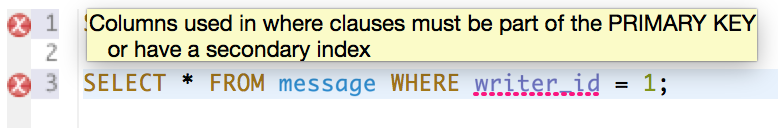
\includegraphics[scale=0.7]{img/where_clause.png}
\caption{Message d'ereur suite à une clause WHERE.}
\end{figure}

\par Ni les rêquetes imbriquées ni les jointures ne sont pérmises en CQL. 
On propose donc l'implémentation suivante en 2 étapes:
\begin{itemize}
\item Recréer une clef composite avec msg\_id et writer\_id comme à la question suivante.
\item Récupérer dans une reqête ultérieur les identifiants des utilisateurs suivits par george.
\end{itemize}

On obtient le résultat suivant:

\begin{figure}[ht]
\centering
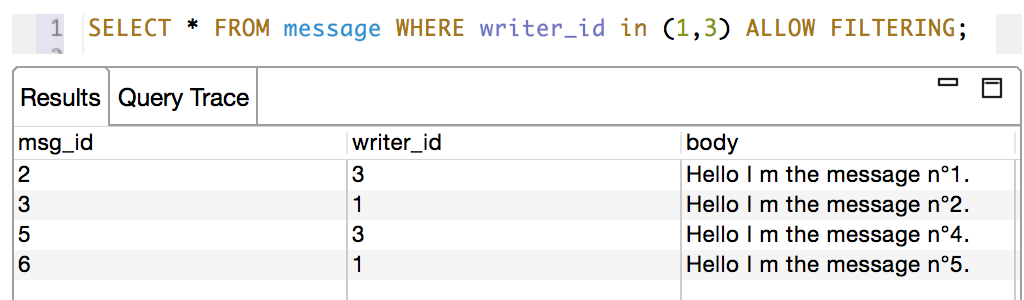
\includegraphics[scale=0.7]{img/george_time_line.png}
\caption{Time line de George.}
\end{figure}

\begin{block}{Conclusion}
Pour plusieur raison l'oppération proposée n'est pas satiffaisante.
Dans un premier temps le changement de contrainte autorise des messages de même identifiant si 
l'émetteur du message est différent. Le manque de requête imbriquée nous force à écrire 
les attributs de la clause WHERE à la main (1,3). Et enfin même avec cette astuce Cassandra indique que 
cette requête ne peut pas être effectuée pour des raisons de performance. On doit alors autoriser 
le filtrage à l'aide de l'instruction \textcolor{cyan}{ALLOW FILTERING}. \newline

En somme, comme beacoup de question en NoSQL, la solotion 
doit être gérée applicativement. C'est à dire dans le code de l'application qui fait appel à Cassandra 
et non dans la partie persistence du système.

\end{block}

\subsection{API python}
Pour revenir sur la question de la timeline nous proposons de passer par un langage de programation en installant
le connecteur Cassandra associé. La documentation du package Cassandra pour python sur \href{https://datastax.github.io/python-driver/}{\textcolor{cyan}{\underline{le site}}} de datastax.
\begin{block}{téléchargement} \href{https://pypi.python.org/pypi/cassandra-driver/}{https://pypi.python.org/pypi/cassandra-driver/2.6.0c2}\end{block}
Pour l'intallation réalise la comande suivante sur le serveur ou se trouve la base de donnée.
On ouvre ensuite IPython notebook, éditeur et l'on repport le code ci-dessous.
\begin{tt}\$ pip install cassandra-driver \end{tt}

\begin{figure}[ht]

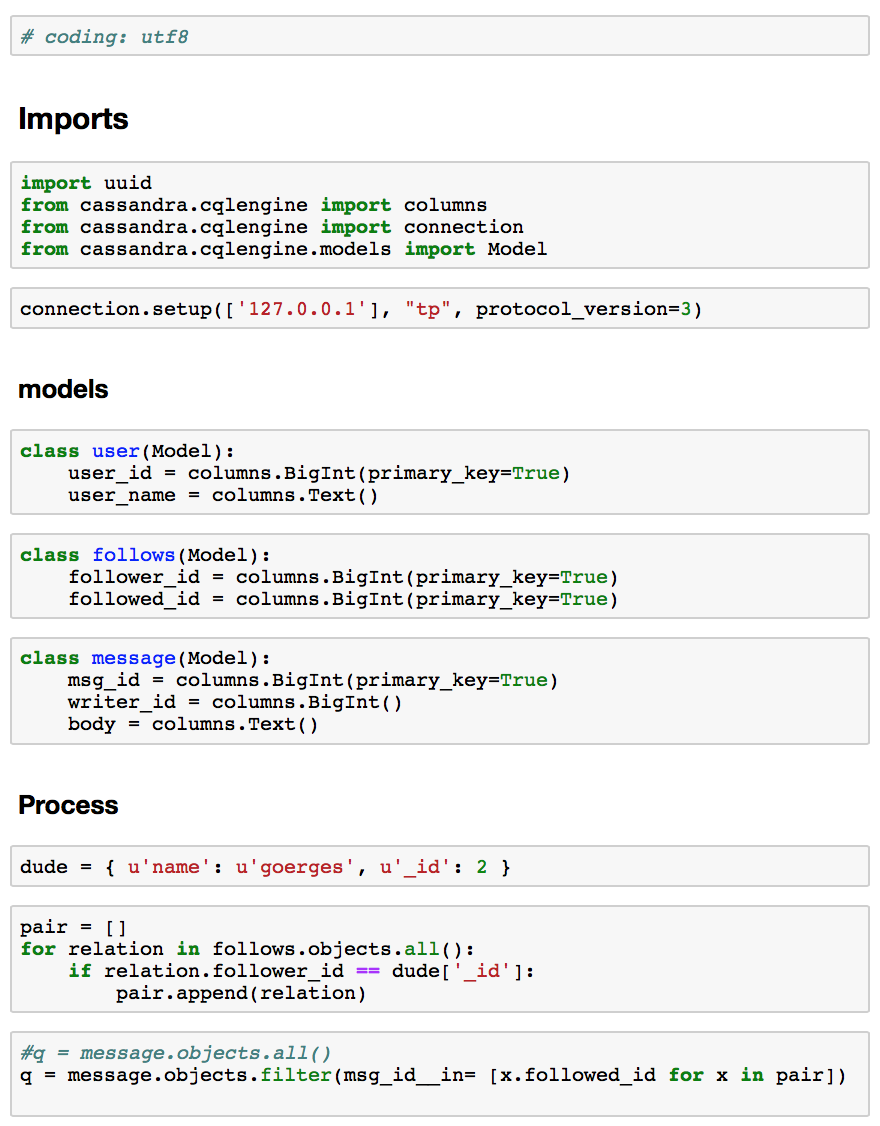
\includegraphics[scale=0.9]{img/ipython.png}
\caption{Ipython notebook.}
\end{figure}

\subsection{Mini Twitter}